


\begin{abstract}
Conservation laws have many applications in numerical relativity. However, it is not straightforward to define local conservation laws for general dynamic spacetimes due the lack of coordinate translation symmetries. In flat space, the rate of change of energy-momentum within a finite spacelike volume is equivalent to the flux integrated over the surface of this volume; for general spacetimes it is necesary to include a volume integral of a source term arising from spacetime curvature. In this work, a study of continuity of matter in general relativity is extended to include angular momentum of matter and Noether currents associated with gauge symmetries. Expressions for the Noether charge and flux of complex scalar fields and complex Proca fields are found using this formalism. Angular momentum density, flux and source are also derived which are then applied to a numerical relativity collision of boson stars in 3D with non-zero impact parameter. A convergence analysis of the numerical simulation shows the conservation system to be obeyed in the continuum limit. [IS THIS LAST SENTANCE NEEDED?]  

\end{abstract}
%\pacs{}






%%%%%%%%%%%%%%%%%%%%%%%%%%%%%%%%%%%%%%%%%%%%%%%%%%%%%%%%%%%%%%%%%%
\subsubsection*{Conventions}

Throughout this work the metric has sign $\{-,+,+,+\}$ and physical quantities will be expressed as a dimensionless ratio of the Planck length $L_{pl}$, time $T_{pl}$ and mass $M_{pl}$ unless stated otherwise; for example Newtons equation of gravity would be written as
\begin{equation}
F=\frac{GMm}{r^2} \quad \rightarrow \quad\left(\frac{F}{F_{pl}}\right) = \frac{\left(\frac{M}{M_{pl}}\right)  \left(\frac{m}{M_{pl}}\right)}{\left(\frac{r}{L_{pl}}\right)^2},
\end{equation}
where $F_{pl} = M_{pl}L_{pl}T_{pl}^{-2}$ is the Planck force. Consequently $c$, $G$ and $\hbar$ take the numerical value of $1$. Additionally, tensor fields will be denoted using bold font for index free notation and normal font for the components. The dot product between two vector fields will be written interchangeably as $\bs{A}\cdot\bs{B}\leftrightarrow A^\mu B_\mu$ for readability. Finally, $\bs\nabla$ represents the covariant derivative and $\partial_i$ is the partial derivative with respect to coordiante $x^i$.
\section{Introduction} \label{sect:intro}


Conservation laws play an important role in many areas of physics. For a general Lagrangian density $\mathcal{L}$, dependant on fields $\phi_i$ and derivatives $\partial_k \phi_i$, if a transformation $\phi_i \rightarrow \phi_i + \delta \phi_i$ leaves the Lagrangian constant the Euler-Lagrange equations imply there is a conserved current $\boldsymbol{J}$,
\begin{equation}
J^k = \sum_i \frac{\partial \mathcal{L}}{\partial (\partial_k \phi_i)}\delta \phi_i.
\end{equation}
In curved space a conserved current $\bs{J}$ satisfies $\nabla_\mu J^\mu = 0$. For some instance in time a charge $Q$, within volume $V$, can be associated with $\bs{J}$ along with a flux ${F}$ through the 2-surface $\partial V$, the boundary of $V$. If the $\bs{J}$ is conserved then $Q$ is a conserved charge satisfying
\begin{equation}
\label{first_qf}\partial_t Q = {F}.
\end{equation}
This says the rate of change of a charge in a volume $V$ is equal to the flux across the boundary $\partial V$ of $V$. In the case that $\bs{J}$ has a non-zero divergence, $\nabla_\mu J^\mu \neq 0$, Eq.~(\ref{first_qf}) generalises to the continuity equation
\begin{equation}
\label{first_qfs}\partial_t {Q} = {F} - {S}.
\end{equation}
In Eq.~(\ref{first_qfs}), ${S}$ is the source of $\bs{J}$ in volume $V$ which can be understood as the destruction or creation of charge $Q$. Eq.~(\ref{first_qfs}) is a simplified version of Eq.~(\ref{qfs_system}), later referred to as the QFS system.


Measurements of the continuity equations above, and their corresponding charges ${Q}$, have many uses in Numerical Relativity. One such use is the measurement of the Noether current $\bs{J}$ of a complex scalar/vector field which arises from a $U(1)$ gauge symmetry of the matter fields $\psi_j$ of the form $\psi_j \rightarrow \psi_j e^{ia} \sim \psi_j + i a \psi_j$ for some small constant $a$. The total charge $Q$, also called Noether charge, is useful to track during numerical simulations as it gives insight into the numerical quality of a simulation. A violation of Noether charge conservation can arise from insufficient resolution in some region of the simulation or due to boundary conditions in a finite volume simulation. In the case of Sommerfeld (outgoing wave) boundary conditions \cite{Alcubierre:2002kk} we might expect charge to be transported out of a finite simulation domain and the total charge $Q$ in the simulation should decrease. Monitoring only ${Q}$ it is impossible to tell whether Noether charge violation is due to a flux ${F}$ through the surface $\partial V$ or undesirable numerical inaccuracies. It is more useful to check whether continuity Eq.~(\ref{first_qf}) (or equivalently Eq.~(\ref{first_qfs}) if there were a non-zero source term) is obeyed for a finite domain $V$; if this fails there is likely a problem as the continuity equations should be exactly observed for general spacetimes. 

When dealing with black hole spacetimes resolution requirements typically become very strict towards the singularity and lead to a local violation of Eqs.~(\ref{first_qf}) and (\ref{first_qfs}). This might not doom a simulation as most physical applications in GR have singularities contained by an event horizon and are causally disconnected from the rest of the simulation; a resolution problem in the vicinity of a singularity therefore will likely not propogate to the exterior. It could be helpful instead to consider a volume $\bar{V}$ equal to $V$ but removing a set of finite volumes $\tilde{V}_i$ which surround any singularities and are preferably comfortably inside any event horizons. Testing Eqs.~(\ref{first_qf}) and (\ref{first_qfs}) in volume $\bar{V}$ would then give a measure of the simulation resolution untainted by the resolution issues at a singularity.

Another use of the continuity equations is to measure the amount of energy-momentum belonging to matter fields within a volume $V$. This has many possible applications such as calculating the total energy or momentum of compact objects like stars. In this paper we are interested in the continuity of angular momentum and apply the analytic results [EXPAND?] to the numerically simulated spacetime of a compact object formed from the collision of two boson stars. The energy-momentum of matter obeys a conservation law in General Relativity as given by by Roger Penrose \cite{10.2307/2397365} where the considered spacetime was assumed to admit a Killing vector. In the case a Killing vector exists then a conserved current $\bs{J}$ associated with the energy-momentum tensor $\bs{T}$ can be identified. The current is $J^\mu = T^\mu_\nu \xi^\nu$ for some Killing vector $\bs{\xi}$ and satisfies $\nabla_\mu J^\mu = 0$. If $\bs{\xi}$ is a Killing vector then Eq.~(\ref{first_qf}) is the correct continuity equation and the charge $Q$ is conserved. In General Relativity the existence of Killing vectors is rare, reserved for spacetimes with special symmetries. Generic dynamic spacetimes with no symmetries, such as in-spirals and grazing collisions of compact objects, have no easily identifiable Killing vector fields. In the case there is no Killing vector the divergence of $\bs{J}$ becomes $\nabla_\mu J^\mu = T^{\mu\nu}\nabla_\mu \xi_\nu$ and the source term ${S}$ is non-zero. Now Eq.~(\ref{first_qfs}) is the correct continuity equation and the charge $Q$ is no longer conserved. Section \ref{sect:mattercont} shows how the choice of $\bs{\xi}$ effects the type of current $\bs{J}$, and therefore charge $Q$, obtained. While measures of energy or momentum are interesting in their own right, the measure of Eq.~(\ref{first_qfs}) within some singularity free finite volume $\bar{V}$ can be a good measure of numerical quality of a simulation in a similar fashion to the measure of Noether charge mentioned already. 

[MAKE THIS LESS AGRESSIVE, ADD SOME MORE REFS LIKE THOMAS] Currently in Numerical Relativity it is common to measure energy, momentum or angular momentum in a localised region with the charge ${Q}$, for instance \cite{Sanchis_Gual_2019}, \cite{Di_Giovanni_2020}. While this is a good measure it doesn't tell the whole story. [SMTH ABOUT PERFECT CONSERVATION IF KILLING VECTOR AND NOT IF NOT]. Other popular methods to obtain energy-momentum of a system include integrating asymptotic quantities such as ADM mass and momentum, however these can't be used locally as they are defined in the limit of large radii only.

Recent work by K. Clough \cite{clough2021continuity} evaluates $Q$, $F$ and $S$ for energy and linear momentum with the assumption that the approximate Killing vector $\bs{\xi}$ is a coordinate basis vector that satisfies ${\partial_i \xi^j} =0$. Successful numerical tests of Eq.~(\ref{first_qfs}) are given for fixed and dynamic background simulations.

This paper builds on the work of \cite{clough2021continuity} and generalises the system to measure angular momentum conservation and the conservation of Noether charges of complex scalar fields and spin-1 complex Proca fields. The assumption that the approximate Killing vector $\bs{\xi}$ is a basis vector satisfying $\partial_i \xi^j = 0$ is dropped and leads to a more general source term $\mathcal{S}$. The QFS system for angular momentum is also tested, using a fully non-linear numerical Relativity simulation, on a spacetime consisting of two boson stars colliding in a grazing fashion.

In section \ref{sect:derive} the QFS system for a general non-conserved current is derived and section \ref{sect:sphere} explicitly expands the results for use with a spherical extraction surface. While no other extraction surfaces are given the results of \ref{sect:sphere} are easily applicable to other shapes. Section \ref{sect:noether} is a standalone derivation of the well known Noether charge density from the QFS perspective and goes on to find the flux variable; results for complex scalar fields and complex Proca fields are given. The application of the QFS system to energy momentum currents, angular momentum and energy are given in section \ref{sect:mattercont}. A fully non-linear test of the QFS system for angular momentum, using GRChombo \cite{clough2015grchombo,Andrade2021} to perform Numerical Relativity simulations, is presented in section \ref{sect:results} along with a convergence analysis.



\section{Derivation of the QFS System} \label{sect:derive}
For a spacetime $(\mathcal{M},\bs{g})$ we start by defining a vector field $\bs{J}$ and subjecting it to the following continuity equation,
\begin{align}
\label{continuity_eqn_def}\nabla_\mu J^\mu = S,
\end{align}
where $S$ is a source term and describes the non-conservation of $\bs{J}$. In the case $S=0$ the current is conserved. We are interested in measuring the charge associated with $\bs{J}$ in a spatial 3-volume $V\in\Sigma$. Here $\Sigma$ is the usual 3-dimensional spacelike manifold $\Sigma$ consisting of the set of all points with constant time coordinate $t$, equipped with metric $\bs{\gamma}$. $\Sigma$ is spanned by spatial coordinates $x^i$ related to the full spacetime coordinates $x^\mu$ by $ x^\mu = \{t,x^i \}$. The boundary of $V$ is a 2-dimensional volume $\partial V$ with metric $\bs{\sigma}$. The normal to $\Sigma$ is the unit co-vector $\bf{n}$ defined as, 
\begin{align}
\label{n_def}
n_\mu :&= \frac{\nabla_\mu t}{\sqrt{g^{\rho\sigma}\nabla_\rho t \nabla_\sigma t}} = -\{\alpha,0,0,0\}, \\
\label{n_def2} n^\mu &= \frac{1}{\alpha}\left(t^\mu - \beta^\mu \right)= \frac{1}{\alpha} \{1, -\beta^i \} , 
\end{align} 
where $(\alpha,\beta^i)$ are the usual lapse and shift from the ADM 3+1 spacetime decomposition \cite{2008}. The reader is directed to \cite{gourgoulhon20073+} for a comprehensive introduction to the $3+1$ decomposition. In Eq.~(\ref{n_def2}), $t^\mu = \{1,0,0,0\}$ is the future directed vector and is distinct from $n^\mu$. Time vector $\bs{t}$ is useful as it's integral curves form lines of constant spatial coordinates. With this knowledge we can define the 4-volume $M$, the spatial 3-volume $V$ evolved along integral curves of $\bs{t}$ between times $t_0\leq t\leq t_0 + \delta t$ in the limit $\delta t\rightarrow 0$. Finally we define the 3-dimensional volume $H$, with metric $h$. $H$ is the evolution of $\partial V$ along integral curves of $\bs{t}$ between times $t_0\leq t \leq t_0 + \delta t$ and is the 3-volume the flux crosses; clearly our definition of $H$ will affect our definition of flux. There is no reason to choose the timelike vector $\bs{t}$, rather than $\bs{n}$, to evolve $V$ and $\partial V$ in time and both will result in a different definition of flux density. It is shown in appendix section \ref{sect:generality} that these two choices result in the same conservation equations. A diagram summarising the relevant geometry can be found in Fig.~\ref{fig:qfs_geometry}.

\begin{figure}[h]
{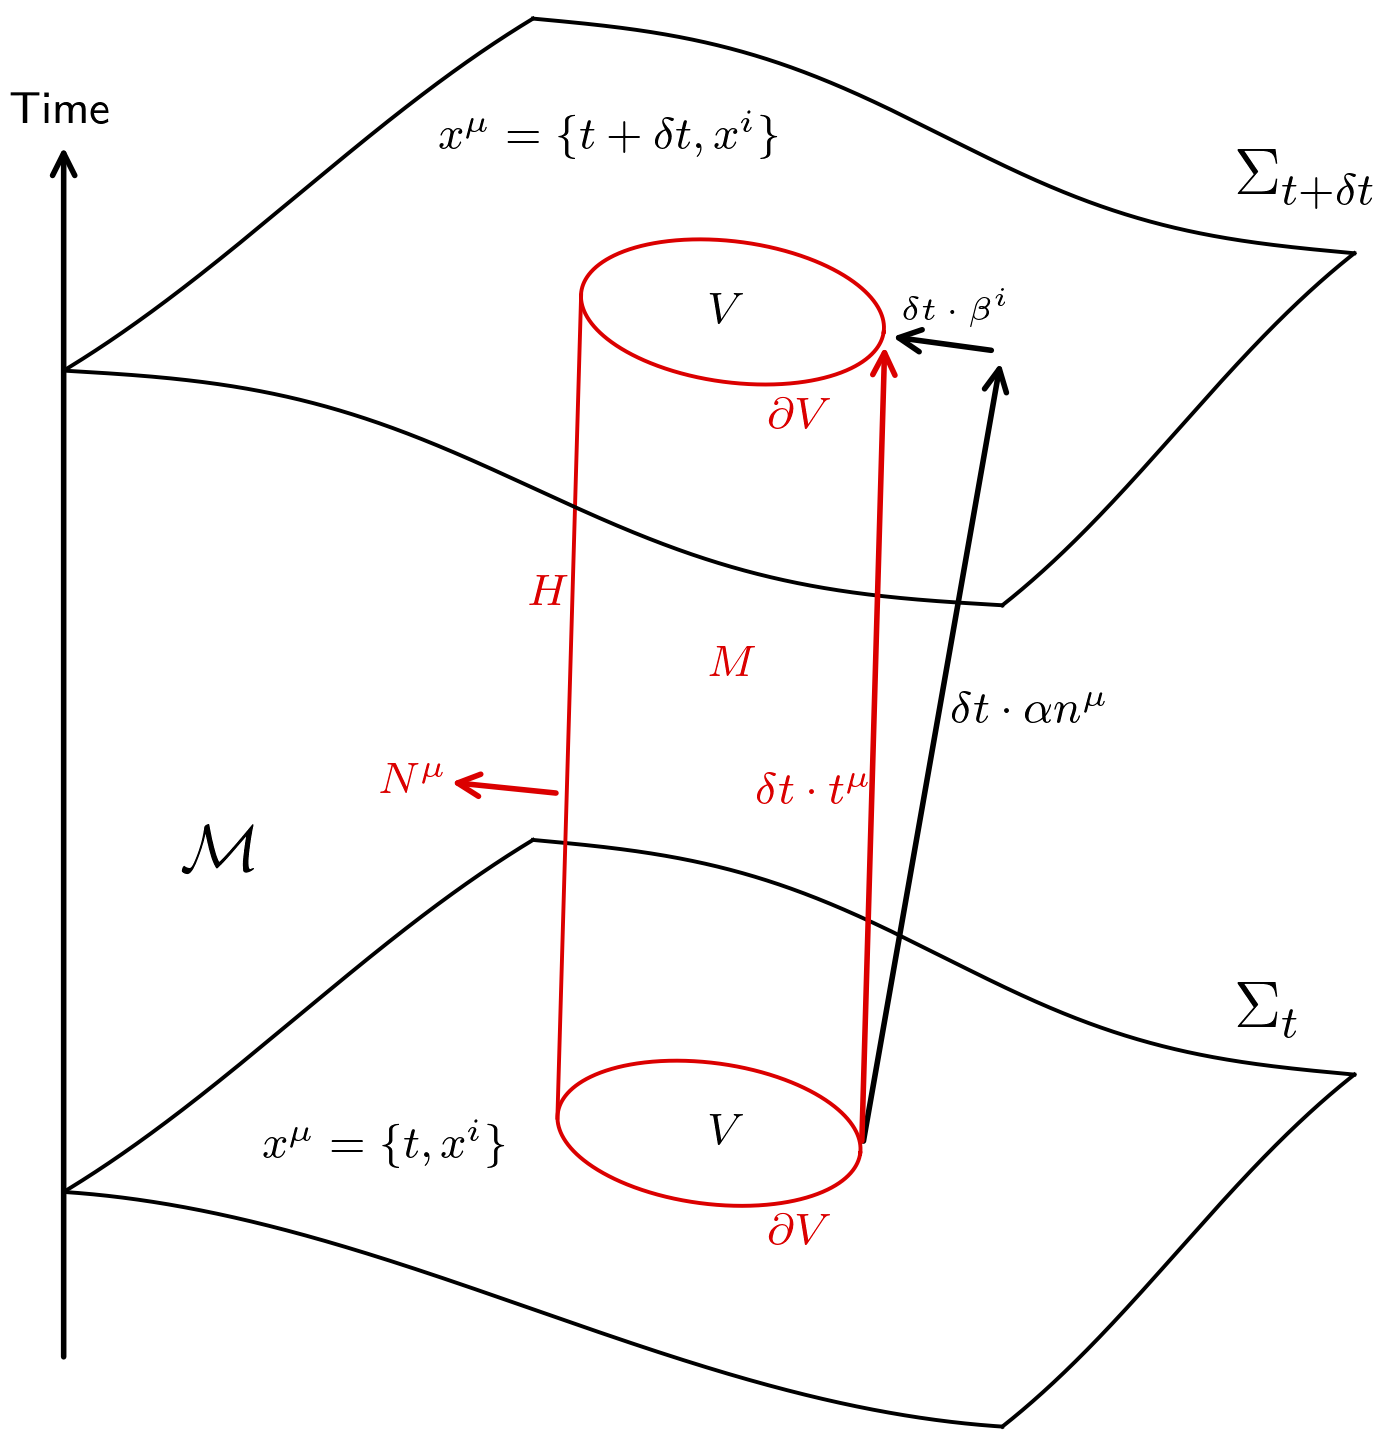
\includegraphics[width=1.0\columnwidth]{qfs_simple.png}}
\caption{Diagram of relevant geometry for derivation of QFS system in section \ref{sect:derive} on manifold $\mathcal{M}$. $\Sigma_t$ is the spatial hypersurface at time $t$ and $\Sigma_{t+\delta t}$ is the the spatial hypersurface at a later time $t+\delta t$. $V$ is the coordinate volume, with surface $\partial V$, that we wish to use as an extraction volume on $\Sigma_t$. The sides of the red cylinder are $H$, defined by $\partial V$ evolved along integral curves of $\bs{t}=\bs{\partial_t}$. The interior of $H$ between times $t$ and $t+\delta t$ is $M$. Evolving $\partial V$ foreward in time with $\bs n$, as demonstrated with the long black arrow, gives a differnet coordinate volume on $\Sigma_{t+\delta t}$ than on $\Sigma_t$.}
\label{fig:qfs_geometry}
\end{figure}

With the relevant geometry discussed we can derive the QFS system, Eq.~(\ref{first_qfs}), by integrating Eq.~(\ref{continuity_eqn_def}) over $M$;
\begin{align} \label{master_integral}
\int_{M } \bs{\nabla}\cdot \bs{J} \sqrt{-g} \;\dd x^4 &= \int_{M } S \sqrt{-g} \;\dd x^4.
\end{align}
Let us start by using Gauss' theorem for curved space \cite{baumgarte_shapiro_2010} on the left hand side, 
\begin{align} \label{master_gauss}
\int_{M } \bs{\nabla}\cdot \bs{J} \;\dd x^4  = \int_{\partial M } \hat{\bs{s}} \cdot \bs{J} \sqrt{{}^{(3)}{g}} \;\dd x^3 ,
\end{align}
with $\sqrt{{}^{(3)}g}$ being the volume element of a generic 3-surface and $\hat{\bs{s}}$ being the corresponding unit normal. This transforms the integral of  $\bs{\nabla} \cdot \bs{J}$ over $M$ to a surface integral of $\bs{J}$ over the compound 3-volume $\partial M$. This surface is split into an integral over $H$ and two integrals over $V$ at times $t_0$ and $t_0 + \delta t$. The integrals over $V$ give,
\begin{align}
&\left(\int^{(t=t_0)}_{V} - \int^{(t=t_0+\delta t)}_{V} \right)\bs{n} \cdot \bs{J} \sqrt{\gamma} \,\dd^3 x ,\nonumber \\
&=-\int_{V}\big[[\bs{n} \cdot \bs{J} \sqrt{\gamma}]_{t+\delta t} - [\bs{n} \cdot \bs{J} \sqrt{\gamma}]_{t}\big] \,\dd^3 x, \\
\label{q_int}&=-\delta t\,\partial_t \int_{V} \bs{n} \cdot \bs{J} \sqrt{\gamma}\,\dd^3 x ,
\end{align} 
where we made use of the fact that the coordinate volume $V$ is constant for all times due to it evolving in time with $t^\mu$. Here $\sqrt{\gamma}$ is the volume element on the spacelike manifold $\Sigma$. Now let us evaluate the integral over $H$, with metric $\bs{h}$ of signature $(-,+,+)$,
\begin{align} 
&\int_{H} \bs{N} \cdot \bs{J} \sqrt{-h} \,\dd^2 x\,\dd t, \nonumber \\
&=\int_{\partial V}  \bs{N} \cdot \bs{J} \sqrt{-h} \,\dd^2 x\int_t^{t+\delta t}\dd t, \\
\label{f_int}&=\delta_t \int_{\partial V} \bs{N} \cdot \bs{J} \sqrt{-h} \,\dd^2 x,
\end{align}
where $\bs{N}$ is the unit normal to $H$ as shown in Fig.~\ref{fig:qfs_geometry}. Given that $\bs{n}$ is not tangent to $H$, but the time vector $\bs{t}$ is, we have $\bs{N} \cdot \bs{n} \neq 0$ and $\bs{N} \cdot \bs{t} =0$. This means we must normalise $\bs{N}$ with metric $\bs{g}$ and not $\bs{\gamma}$ as $\bs{N}$ is not tangent to $\Sigma$ and $\bs{g}(\bs{N},\bs{N})\neq \bs{\gamma}(\bs{N},\bs{N})$. In other words, $\bs{N}$ is a 4-vector in the case we time evolve $V$ with time vector $\bs{t}$ but $\bs{N}$ is a 3-vector if we time evolve with $\bs{n}$. Finally the right hand side source term from (\ref{master_integral}) becomes,
\begin{align}
&\int_{M} S \sqrt{-g} \;\dd x^4 , \nonumber \\
&=\int_V S \sqrt{-g} \;\,\dd x^3 \int_t^{t+\delta t} \dd t,\\
 \label{s_int}&=\delta t \int_V S \alpha\sqrt{\gamma} \;\dd x^3 .
\end{align}
Combining Eqs.~(\ref{q_int}), (\ref{f_int}) and (\ref{s_int}) transforms Eq.~(\ref{master_integral}) into,
\begin{equation} \label{qfs_system}
\partial_t \int_{V} \mathcal{Q} \sqrt{\gamma} \,\dd^3 x  = \int_{\partial V} \mathcal{F} \sqrt{\sigma} \,\dd^2 x  
 - \int_{V} \mathcal{S} \sqrt{\gamma} \,\dd^3 x,
\end{equation}
where the density, flux density and source density ($\mathcal{Q}, \mathcal{F}, \mathcal{S}$) of angular momentum are defined as,
\begin{align}
\label{q_def}\mathcal{Q} :&= J^\mu n_\mu , \\
\label{flux_def}\mathcal{F} :&= \frac{\sqrt{-h}}{\sqrt{\sigma}}J^\mu N_\mu , \\
\label{source_def}\mathcal{S} :&= \alpha S. 
\end{align} 
For later sections it is useful to split the normal vector $\bs{N}$ into its spacelike and timelike parts,
\begin{align}
\label{3plus1n}N_\mu = \pN_\mu - \bs{n} \cdot \bs{N} n_\mu,
\end{align}
where $\pN_\mu = \perp^\nu_\mu N_\nu$ is the projected part of $\bs{N}$ onto $\Sigma$ with $\bs{n}\cdot \bs{\pN}=0$ and $\bs{\perp}$ is the projection operator onto $\Sigma$,
\begin{align}
\label{perp} \perp^\nu_\mu = \delta^\nu_\mu + n^\mu n_\nu.
\end{align}
Using Eqs.~(\ref{3plus1n}) and (\ref{perp}) the flux term becomes, 
\begin{align}
\mathcal{F} &= \frac{\sqrt{-h}}{\sqrt{\sigma}}J^\mu (\pN_\mu - \bs{n} \cdot \bs{N} n_\mu), \\
  \label{3plus1f} &= \frac{\sqrt{-h}}{\sqrt{\sigma}} (\gamma^{\mu\nu} J_\mu N_\nu - \bs{n} \cdot \bs{N} \mathcal{Q}).
\end{align}
The term on the left arises from flux through the surface $\partial V$ and the term on the right is a consequence of the coordinate volume $V$ moving with respect to a normal observer with worldline traced by $\bs{n}$. Writing the flux term as above makes it obvious how the definition of flux depends on the 3-volume $H$ which determines $\sqrt{-h}$, $\sqrt{\sigma}$ and $\bs{N}$. Equivalently it can be seen that the density (\ref{q_def}) and source (\ref{source_def}) terms do not depend on the extraction surface.

\section{Application to Spherical extraction} \label{sect:sphere}
The numerical test in section \ref{sect:results} chooses a spherical volume to extract the angular momentum flux. Using standard Cartesian and spherical polar coordinates, $x^i_{\rm{cart}} = \{x,y,z\}$ and $x^i=\{r,\theta,\phi\}$ respectively, we can define $H$ as the coordinate volume $r=r_0$, $t_0\leq t \leq t+\delta t$. Thus, the normal $\bs{N}$ to $H$ is proportional to $\bs{\nabla}(r-r_0) = \bs{\nabla}(\sqrt{x^2 + y^2 + z^2})$. Explicitly calculating the components $N_\mu$, and normalising to unity, with spherical polar spacelike coordinates gives,
\begin{align}
N_\mu &= \frac{\nabla_\mu r}{\sqrt{g^{\rho\sigma} \nabla_\rho r \nabla_\sigma r}}, \\
     \label{radial_N} &= \frac{1}{\sqrt{g^{rr}}}\{0,1,0,0\}.
\end{align}
Note that if we had chosen $H$ to be $\partial V$ evolved along the unit vector $\bs{n}$ rather than time vector $\bs{t}$ then we would have obtained a different definition of $\bs{N}$ that's perpendicular to $\bs{n}$ rather than $\bs{t}$. The consequences of the alternate choice of $H$ are explored in appendix \ref{sect:generality}.



The density and source terms, $\mathcal{Q}$ and $\mathcal{S}$, do not depend on the choice of surface so we can move on to the flux term. The expansion of the Flux term requires the evaluation of the volume element $\sqrt{-h}$ of $H$. Due to the choice that $H$ is the surface of constant radial coordinate, finding the metric of this surface is straightforward. Here we define spherical polar coordinates $x^\mu = \{t,r,\theta, \phi \}$ on $\mathcal{M}$ and $X^M = \{t,\theta, \phi \}$ spanning $H$. The line element of a curve residing in $H$ can be evaluated in $\mathcal{M}$ or $H$ and must agree,
\begin{align}
\label{induced_metric}h_{MN} \, \dd X^M \dd X^N &= (g_{\mu\nu} - N_\mu N_\nu) \,\dd x^\mu \dd x^\nu, \\
 h_{MN} &= \begin{pmatrix} g_{tt} & g_{t\theta} & g_{t\phi} \\ g_{\theta t} &  g_{\theta\theta}& g_{\theta\phi} \\ g_{\phi t} & g_{\phi\theta} & g_{\phi\phi} \end{pmatrix}.
\end{align}
A similar argument can be made for $\partial V$, the set of all points satisfying $r=r_0$ and $t=t_0$, with metric $\bs{\sigma}$.
\begin{align}
\label{sigma metric}\sigma_{ab} &= \begin{pmatrix} g_{\theta\theta} & g_{\theta\phi} \\ g_{\phi\theta} & g_{\phi\phi} \end{pmatrix} \\
\label{sigma det}\sqrt{\sigma}  &= \sqrt{g_{\theta\theta}g_{\phi\phi} - g_{\phi\theta}g_{\theta\phi}}
\end{align}
Finally, using Cramer's rule for the inverse of a matrix,
\begin{align}
h^{tt} = \frac{{\sigma}}{h},
\end{align}
and reading the $tt$ component of (\ref{induced_metric}), 
\begin{align}
h^{tt} &=      g^{tt} - N^t N^t, \\
               &= -\frac{1}{\alpha^2}\left(\frac{\gamma^{rr}}{g^{rr}} \right), 
\end{align}
we can relate $\sqrt{\sigma}$ and $\sqrt{-h}$,
\begin{align}
     \label{rootminushexpand}\sqrt{-h} = \alpha \sqrt{\sigma} \sqrt{\frac{g^{rr}}{\gamma^{rr}}}.
\end{align}
Using this with Eq.~(\ref{radial_N}) we can expand Eq.~(\ref{flux_def}) for the flux term $\mathcal{F}$, 
\begin{align}
 \label{spherical_flux}\mathcal{F}&=  \frac{\sqrt{-h}}{\sqrt{\sigma}} J^\mu N_\mu = \frac{\alpha}{\sqrt{\gamma^{rr}}} J^r, 
 \end{align}
 but for practical purposes it is helpful to decompose this in terms of 3+1 variables as in Eq.~(\ref{3plus1f}),
 \begin{align}
   \mathcal{F} &= \alpha\frac{\sqrt{g^{rr}}}{\sqrt{\gamma^{rr}}} \left(\gamma^{\mu\nu}J_\nu {N}_\mu - \bs{n} \cdot \bs{N} \mathcal{Q}\right), \\
                   &=  \alpha\frac{\sqrt{g^{rr}}}{\sqrt{\gamma^{rr}}}\left(\gamma^{r\nu}J_\nu \frac{1}{\sqrt{g^{rr}}} +\alpha^{-1}\beta^r\frac{1}{\sqrt{g^{rr}}} \mathcal{Q}\right), \\
\label{3plus1fluxspherical}   &= \frac{1}{\sqrt{\gamma^{rr}}}\left(\alpha\gamma^{r\nu}J_\nu  + \beta^r \mathcal{Q}\right).
\end{align}
It is straightforward to re-derive these results for other extraction volume shapes, such as cylinders or cubes/rectangles, with a redefinition of spacelike volume $V$ giving rise to different $\bs{N}$, $H$ and $\partial V$. It is wise to pick suitable coordinates adapted to the symmetry of the problem.

\section{Noether Currents} \label{sect:noether}

In this section we apply the previous results of the QFS system Eq.~(\ref{qfs_system})
to the continuity of Noether charge for both a complex scalar and the Proca field. The charge $\mathcal{Q}$ represents the number density of particles. Since the total particle number minus antiparticle number is always conserved the conservation law is exact and the source term $\mathcal{S}$ vanishes. 

Globally the total Noether charge should be conserved, however in numerical simulation this might not always be the case. Two common ways for non-conservation to occur are for the matter to interact with the simulation boundary conditions (usually unproblematic) or some region of the simulation being insufficiently resolved (often problematic). Without knowledge of the Noether flux it is difficult to know what a change in Noether charge should be attributed to. If a large extraction volume/surface containing the relevant physics shows a violation of Eq.~(\ref{qfs_system}) then the change in total Noether charge being due to boundary conditions can be ruled out and resolution is likely the culprit. 

When considering black hole spacetimes it is common for Noether charge to be dissipated as matter approaches the singularity; this is due to resolution requirements typically becoming very high in this region. The violation of Eq.~(\ref{qfs_system}) inside a black hole horizon might not cause any resolution problems for the black hole exterior however due to causal disconnection. If the extraction volume is modified to exclude finite regions containing any black hole singularities then Eq.~(\ref{qfs_system}) could be used to monitor the conservation of Noether charge away from troublesome singularities. This would be a good way of checking the resolution of a matter field in situations such as boson/Proca stars colliding with black holes or scalar/vector accretion onto a black hole.






